%!TEX root = main.tex

\chapter{Implementation of an entangled database for GSA}
\label{chp:implementation}

In order to give a touch of reality to our research work we would like to present an implementation of the algorithm described in \cref{sec:shift_and_control}. We first provide an implementation in Octave, that simulates the effects of quantum operations through matrix calculation and provides a clear view of the matrices shape. Then we provide an implementation in Q\# through Microsoft QDK.

\section{Octave}
\label{sec:octave_impl}

In this chapter we will implement several operations in Octave, both common ones and ad hoc defined ones. The reader can find the definition of all new introduced gates and operations in \cref{sec:derived_gates}.

In the following we show first a commented version of the output of the algorithm and then the source code.

\lstinputlisting[language=octave, caption={Entangled DB implemented in Octave (output only)}, label={lst:octave_entangled_db_output}]{entangled_db_ouput.txt}

\noindent Octave script (some log commands are omitted for brevity):

\lstinputlisting[language=octave, caption={Entangled DB implemented in Octave (code)}, label={lst:octave_entangled_db}]{entangled_db_script.txt}

\noindent where \textit{switch\_g()} implements the swapping gates described in \cref{tab:switch_gates}.

\section{Q\#}
\label{sec:qs_impl}

Now we would like to implement in a quantum development environment some parts of the Octave code shown in \cref{sec:octave_impl}, we will use Microsoft QDK (described in \cref{chp:qdk}) and the programming language will be Q\#.

\bigskip

\noindent First let's define an operation to set qubits' state to a desired one.

\lstinputlisting[style=qsharp, firstline=6, lastline=12]{../QsharpSolution/PhoneBook/Operations.qs}

\noindent Then let's define a couple of custom gates, like we have done in Octave

\lstinputlisting[style=qsharp, firstline=13, lastline=32]{../QsharpSolution/PhoneBook/Operations.qs}

\noindent And now let's define an useful operator that performs control on \textit{ctrl\_qubits=0}

\lstinputlisting[style=qsharp, firstline=33, lastline=39]{../QsharpSolution/PhoneBook/Operations.qs}

\noindent Finally we can put everything together and implement the Octave code seen in \cref{lst:octave_entangled_db}. To let the reader understand better what's happening we will perform just the first row swap (between rows 1 and 3), but the process for the second swap (between rows 2 and 6) is similar.

\lstinputlisting[style=qsharp, firstline=65, lastline=96, caption={Building the entangled database in Q\#}, label={lst:entangled_db_qs}]{../QsharpSolution/PhoneBook/Operations.qs}

In \cref{fig:row13_swap} we see the row swap between 1 and 3 in action, in particular the outputs when entering $(0,0,0)$ and $(0,1,0)$ are swapped, as it should be.

In \cref{fig:primed_matrix} we see the primed matrix $A'$ (without row swaps). Notice that there is an equal probability of getting 0 or 1 on the least significative qubit when the first 2 are both zero (i.e. H $2 \times 2$ gate has been applied in direct sum with an identity matrix), as it should be.

Finally in \cref{fig:preparation_matrix} we see both operations performed on the same circuit, therefore producing an indetermination on the second least significative qubit as well, which is the changing one between row 1 (000) and row 3 (010).

\begin{figure}
	\centering
	\begin{subfigure}{0.49\linewidth}
		\centering
		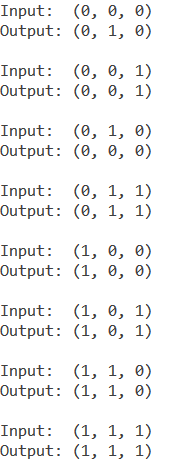
\includegraphics[scale=0.8]{row13_swap}
		\caption{Swap op. between rows 1 and 3}
		\label{fig:row13_swap}
	\end{subfigure}
	\begin{subfigure}{0.49\linewidth}
		\centering
		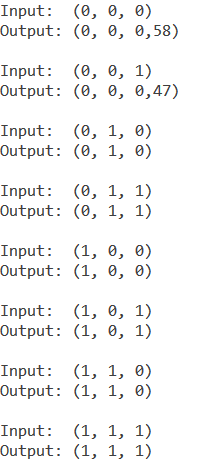
\includegraphics[scale=0.8]{primed_matrix}
		\caption{Primed matrix $A'$}
		\label{fig:primed_matrix}
	\end{subfigure}
	
	\bigskip
	
	\begin{subfigure}{0.5\linewidth}
		\centering
		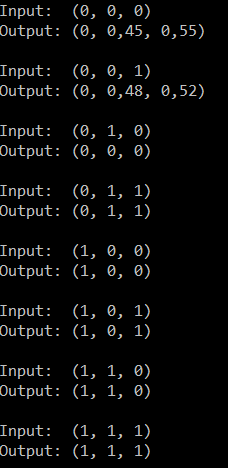
\includegraphics[scale=0.8]{preparation_matrix}
		\caption{Swapped matrix $A$}
		\label{fig:preparation_matrix}
	\end{subfigure}
	
	\caption{Partial outputs of the code in \cref{lst:entangled_db_qs}.}
\end{figure}